\documentclass[12pt]{article}
\usepackage{graphicx}
\usepackage{subcaption}
\usepackage{capt-of}
\begin{document}
\title{Elementaire Statistiek Project}
\author{~E.~Nabil,~20215256\\}
\date{2023-06-19}
\maketitle
\section{Praktische Opdracht}
Schrijf een verslag van maximaal 10 pagina's waarin je de volgende vragen zo volledig mogelijk beantwoordt. 
Geef duidelijk aan welke veronderstellingen worden gemaakt, wat de nul- en alternatieve hypotheses zijn, de conclusie, enzovoort. 
Geef ook de teststatistiek en de waargenomen waarde van de teststatistiek. 
Controleer of de voorwaarden (veronderstellingen) die nodig zijn om de gekozen techniek toe te passen, zijn voldaan. 
Voer de toetsen uit met een significantieniveau van $\alpha = 0,05$.
Voor dit project zullen we gebruikmaken van een dataset. 
De dataset bevat gegevens over eikensoorten die voorkomen in de USA en is te vinden in het bestand "eik.csv". 
De dataset bevat de volgende variabelen:
\begin{enumerate}
    \item \textbf{Boom}: het volgnummer van de beschouwde boomsoort
    \item \textbf{Regio}: de regio waarin de boom voorkomt ('Atlantic' of 'California')
    \item \textbf{Grootte}: de grootte van gebied waarin de soort voorkomt (in 100 km$^2$)
    \item \textbf{Volume}: het volume van de eikel (in cm$^3$)
    \item \textbf{Hoogte}: de hoogte van de boom (in m)
\end{enumerate}
Om ervoor te zorgen dat ik met een unieke dataset werk, moet ik enkele observaties verwijderen op basis van mijn studentnummer. Mijn studentnummer is \textbf{20215256}, dus met de laatste 3 cijfers heb ik \textbf{i = 2}, \textbf{j = 5} en \textbf{k = 6}.
Ik zal de volgende rijen selecteren: $k + 1$, $j + 1$, $i + 1$, $jk + 1$, $ij + 1$, $ik + 1$, $ijk + 1$ en $i + j + k + 1$ uit de dataset.
Dit betekent dat ik de volgende rijen zal verwijderen: 7, 6, 3, 31, 11, 13, 61 en 14.

\newpage
\section{Vragenlijst}
\subsection{Vraag 1}
\textbf{Bestudeer en bespreek de verdeling van de variabelen Volume en Grootte. Bespreek hiertoe gepaste grafische voorstellingen. Ga ook op een formele manier na of de gegevens normaal verdeeld zijn. Indien dit niet het geval is, in welke zin wijken de gegevens af van normaal verdeelde gegevens ? Bespreek ?}
\newline\newline
Om een duidelijk beeld te krijgen van hoe de variabelen verdeeld zijn, heb ik besloten om histogrammen op te stellen voor beide variabelen. 
Een histogram is een visuele weergave waarbij de gegevens worden verdeeld in verschillende "balken" om de frequentie van waarden in elke balk weer te geven. 
Hierdoor kunnen we gemakkelijk de verdeling van de waarden observeren en beoordelen of deze lijkt op een normale verdeling.
\newline\newline
Om de histogrammen nog informatiever te maken, heb ik ervoor gezorgd dat er ook bijpassende normaalcurven worden geplot. 
Een normaalcurve, ook wel bekend als een Gaussische curve of een bell curve, is een wiskundige grafiek die de kenmerken van een normale verdeling weergeeft. 
Door de normaalcurven naast de histogrammen te tonen, kunnen we de verdeling van de variabelen beter beoordelen. 
\newline\newline
Als de waarden in het histogram mooi samenvallen met de vorm van de normaalcurve en een kenmerkende belvorm hebben, wijst dit op een redelijk normale verdeling van de variabelen. 
Als daarentegen de waarden in het histogram niet goed passen bij de vorm van de normaalcurve, kan dit erop duiden dat de variabelen afwijken van een normale verdeling.
Onderaan ziet u de histogrammen voor de variabelen Volume en Grootte.
\newline\newline
% insert histograms for Volume and Grootte
\noindent\begin{minipage}{0.5\linewidth}
    \centering
    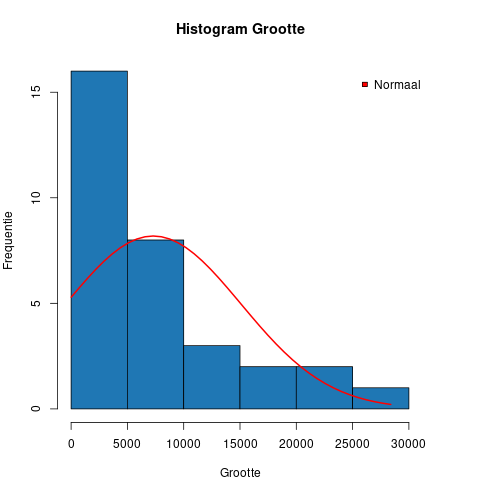
\includegraphics[width=\linewidth]{vragen/vraag1/images/hist_norm_grootte.png}
    \captionof{figure}{Grootte met normale curve.}
    \label{fig:hist_norm_grootte}
\end{minipage}
\noindent\begin{minipage}{0.5\linewidth}
    \centering
    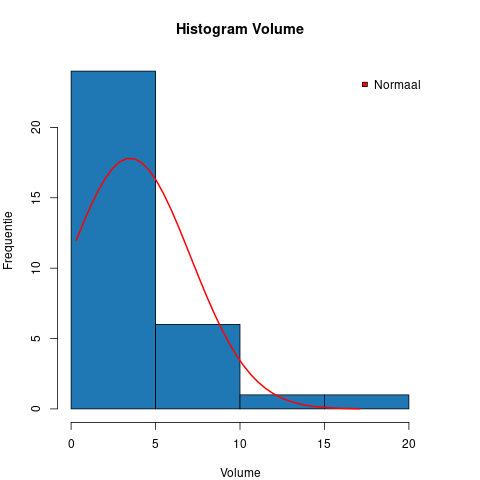
\includegraphics[width=\linewidth]{vragen/vraag1/images/hist_norm_volume.png}
    \captionof{figure}{Volume met normale curve.}
    \label{fig:hist_norm_volume}
\end{minipage}
\newline\newline\newline  
\textbf{Conclusie:} Bij het analyseren van figuur \ref{fig:hist_norm_grootte} en \ref{fig:hist_norm_volume} is me opgevallen dat beide histogrammen leunen aan de linkerkant. 
Dit patroon wordt ook weerspiegeld in de vorm van de bijbehorende normale kromme. 
De piek van de normale kromme verschijnt aan de linkerkant van het histogram en niet in het midden, wat aangeeft dat de gegevens niet normaal verdeeld zijn.
Deze observatie suggereert dat de gegevens mogelijk een asymmetrische verdeling hebben, waarbij de waarden zich concentreren aan de linkerkant en uitwaaieren naar rechts. 
Het kan wijzen op een scheve of skewed verdeling waarin de gemiddelde waarde verschoven is ten opzichte van het midden van de verdeling.
\newline\newline
Ik heb ook een Boxplot opgesteld voor beide variabelen. Dit is een grafiek die een snelle samenvatting geeft van een of meer numerieke variabelen.
De boxplot toont de verdeling van de gegevens op basis van een vijf getallen samenvatting: minimum, eerste kwartiel, mediaan, derde kwartiel en maximum.
Onderaan ziet u de boxplots voor de variabelen Volume en Grootte.
\newline\newline
% insert boxplots for Volume and Grootte
\noindent\begin{minipage}{0.5\linewidth}
    \centering
    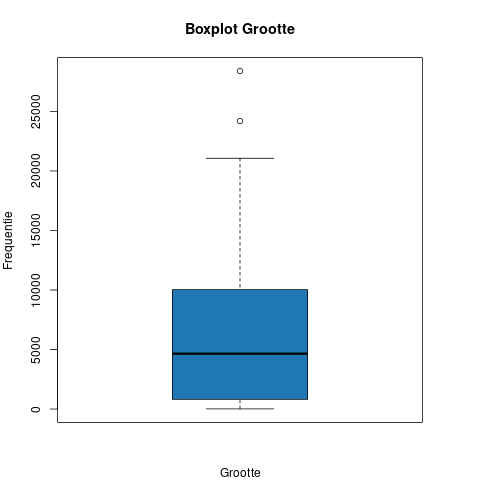
\includegraphics[width=\linewidth]{vragen/vraag1/images/box_grootte.png}
    \captionof{figure}{Boxplot voor Grootte.}
    \label{fig:boxplot_grootte}
\end{minipage}
\noindent\begin{minipage}{0.5\linewidth}
    \centering
    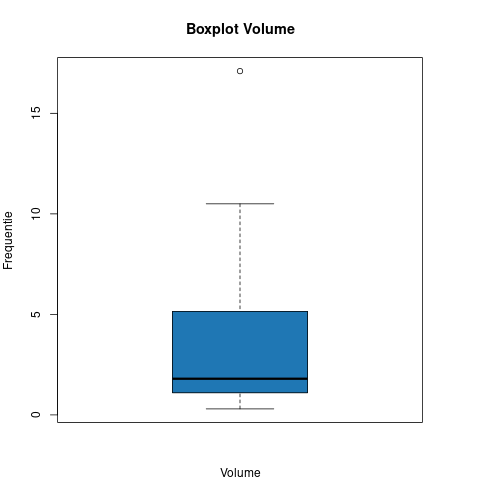
\includegraphics[width=\linewidth]{vragen/vraag1/images/box_volume.png}
    \captionof{figure}{Boxplot voor Volume.}
    \label{fig:boxplot_volume}
\end{minipage}
Als het normaal verdeeld is, zal de mediaan (tweede kwartiel) in het midden van de boxplot liggen.
Ook zal de "whishker" aan beide kanten van de boxplot ongeveer even lang zijn. 
Hieronder een voorbeeld van een boxplot met een normaal verdeelde variabele.
% example of boxplot
\newline\newline
\noindent\begin{minipage}{0.5\linewidth}
    \centering
    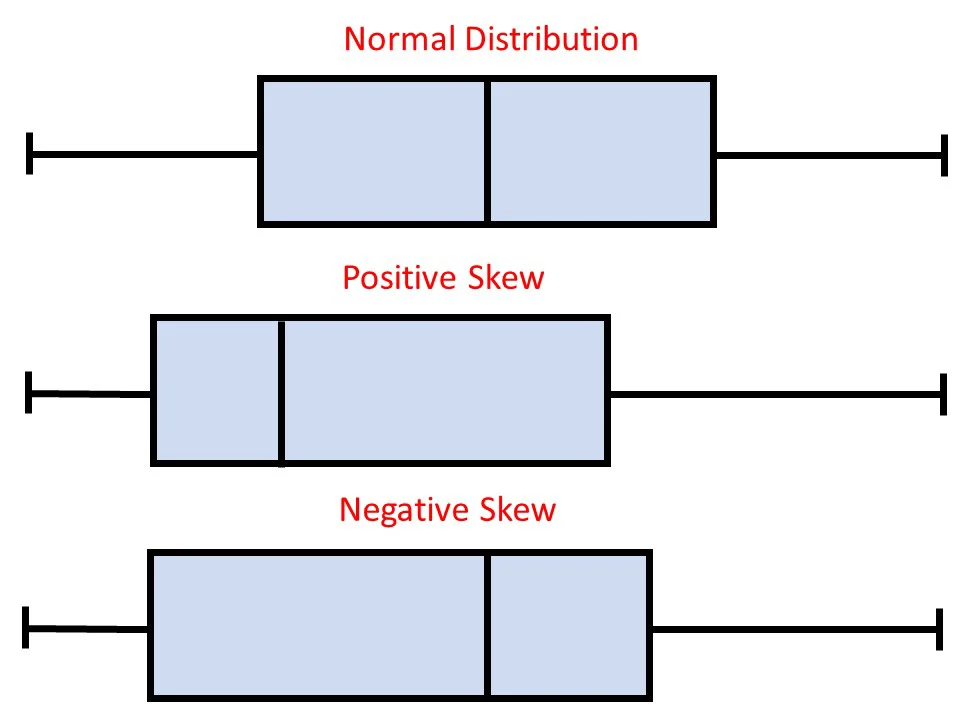
\includegraphics[width=\linewidth]{vragen/vraag1/images/boxplots.png}
    \captionof{figure}{Boxplot referentie.}
    \label{fig:boxplot_ref}
\end{minipage}
\newline\newline
Hier zien we dus dat het niet het geval is voor beide variabelen.
\newline\newline
Om dubbel te controleren of de gegevens normaal verdeeld zijn, heb ik ook een Q-Q plot opgesteld voor beide variabelen.
Een Q-Q plot is een grafiek die de kwantielen van een gegevensverzameling vergelijkt met de kwantielen van een referentieverdeling.
De kwantielen van een verdeling zijn de waarden die de verdeling in gelijke delen verdelen.
\newline\newline
Als de gegevens normaal verdeeld zijn, zullen de punten op de Q-Q plot ongeveer op een rechte lijn liggen.
Als de punten niet op een rechte lijn liggen, kan dit erop duiden dat de gegevens niet normaal verdeeld zijn.
Onderaan ziet u de Q-Q plots voor de variabelen Volume en Grootte.
\newline\newline
% insert qq plots for Volume and Grootte
\noindent\begin{minipage}{0.5\linewidth}
    \centering
    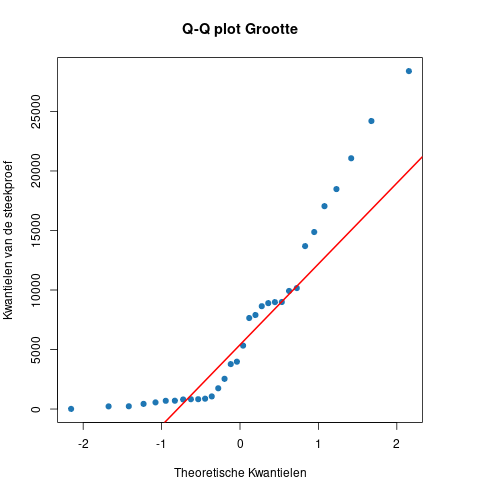
\includegraphics[width=\linewidth]{vragen/vraag1/images/qq_grootte.png}
    \captionof{figure}{Q-Q plot van Grootte.}
    \label{fig:qq_grootte}
\end{minipage}
\noindent\begin{minipage}{0.5\linewidth}
    \centering
    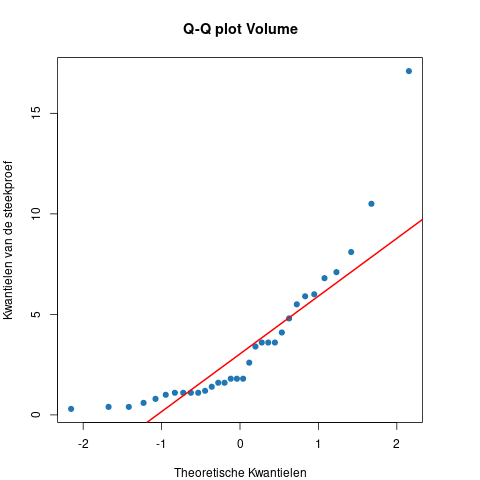
\includegraphics[width=\linewidth]{vragen/vraag1/images/qq_volume.png}
    \captionof{figure}{Q-Q plot van Volume.}
    \label{fig:qq_volume}
\end{minipage}
\newline\newline\newline
\textbf{Conclusie:} Bij het analyseren van figuur \ref{fig:qq_grootte} em \ref{fig:qq_volume} is mij opgevallen dat de punten op de Q-Q plot niet op een rechte lijn liggen.
Dit suggereert dat de gegevens niet normaal verdeeld zijn.
Deze observatie bevestigt mijn eerdere observatie dat de gegevens mogelijk een asymmetrische verdeling hebben, waarbij de waarden zich concentreren aan de linkerkant en uitwaaieren naar rechts.
\newline\newline
Om mijn observaties te bevestigen, heb ik ook de skewness en kurtosis van beide variabelen berekend.
Skewness is een statistische maatstaf die de symmetrie van de verdeling van een variabele meet.
Kurtosis is een statistische maatstaf die de vorm van de verdeling van een variabele meet.
\newline\newline
Als de skewness van een verdeling gelijk is aan 0, is de verdeling symmetrisch.
Als de skewness van een verdeling groter is dan 0, is de verdeling scheef naar rechts.
Als de skewness van een verdeling kleiner is dan 0, is de verdeling scheef naar links.
\newline\newline
Als de kurtosis van een verdeling gelijk is aan 0, is de verdeling normaal.
Als de kurtosis van een verdeling groter is dan 0, is de verdeling zwaarstaartig.
Als de kurtosis van een verdeling kleiner is dan 0, is de verdeling lichtstaartig.
\newline\newline
Onderaan ziet u de skewness en kurtosis van beide variabelen.
\newline\newline
% insert skewness and kurtosis for Volume and Grootte
\begin{tabular}{l*{6}{c}r}
    & Grootte & Volume \\
    \hline
    Skewness & 1.05 & 1.92 \\
    Kurtosis & 0.14 & 4.24 \\
\end{tabular}
\newline\newline\newline
\textbf{Conclusie:} Op het tabel zie je dat de skewness van beide variabelen groter is dan 0.
Dit suggereert dat de verdeling van beide variabelen scheef naar rechts is.
Dit komt overeen met figuur \ref{fig:hist_norm_grootte} en \ref{fig:hist_norm_volume}
\newline\newline
Bij het tabel zie je ook dat de kurtosis van "Grootte" bijna 0 is en de kurtosis van "Volume" groter is dan 0.
Dit suggereert dat de verdeling van beide variabelen zwaarstaartig is.
Dit komt overeen met wat we eerder hebben gezien.
\newline\newline
Als Laatste heb ik ook de Shapiro-Wilk test uitgevoerd.
De Shapiro-Wilk test is een statistische test die wordt gebruikt om te bepalen of een gegevensverzameling normaal verdeeld is.
\newline\newline
De nulhypothese van de Shapiro-Wilk test is dat de gegevens normaal verdeeld zijn.
De alternatieve hypothese van de Shapiro-Wilk test is dat de gegevens niet normaal verdeeld zijn.
\newline\newline
Onderaan ziet u de resultaten van de Shapiro-Wilk test voor beide variabelen.
\newline\newline
% insert shapiro wilk test for Volume and Grootte
\begin{tabular}{l*{6}{c}r}
   & Grootte & Volume \\
   \hline
   Shapiro Wilk & 0.0003 (not normal) & 1.6729e-05 (not normal) \\
\end{tabular}
\newline\newline\newline
\textbf{Conclusie:} Hier merk je dat de p-waarde van beide variabelen kleiner is dan 0.05.
Dit suggereert dat de gegevens niet normaal verdeeld zijn. We kunnen de nullhypothese verwerpen.
Alles duidt erop dat de gegevens niet normaal verdeeld zijn.
We kunnen dus nu vanuit gaan dat de gegevens \textbf{niet} normaal verdeeld zijn.
\newline\newline
\textbf{Extra:}
Wat maakt de gegevens nu wel normaal verdeeld?
Als we de gegevens transformeren, kunnen we proberen de gegevens normaal verdeeld maken.
\newline\newline
Voor de variabele "Grootte" heb ik de vierde machtswortel genomen.
Want dit zorgde voor de grootste Shapiro-Wilk p-waarde.
Voor de variabele "Volume" heb ik de logaritme genomen.
Ook hier zorgde dit voor de beste resultaat.
\newline\newline
Onderaan ziet u tabel voor de skewness, kurtosis en Shapiro-wilk test van beide variabelen na de transformatie.
\newline\newline
% insert Groote and Volume after transformation
\begin{tabular}{l*{6}{c}r}
   \textbf{NA transformatie} & Grootte & Volume \\
   \hline
    Skewness & -0.09 & -0.05 \\
    Kurtosis & -1.24 & -0.86 \\
   Shapiro Wilk & 0.138 (normal) & 0.714 (normal) \\
\end{tabular}
\newline\newline\newline
\textbf{Conclusie:} Zoals je kan zien is de skewness van beide variabelen bijna 0.
Dit betekent dat de verdeling van beide variabelen ongeveer symmetrisch is. Voorheen was het voor "Grootte" 1.05 en voor "Volume" 1.92.
Ten slotte voor de Shapiro-wilk test is de p-waarde van "Volume" en "Grootte" groter dan 0.05.
Voor "Volume" is de logaritme een goede transformatie en is de verdeling normaal verdeeld.
Voor "Grootte" is de vierde machtswortel een goede transformatie en is de verdeling normaal verdeeld.
\subsection{Vraag 2}
\textbf{Ga na of er een verband is tussen dikke eikels, dit zijn eiken waarvan het volume van de eikel minstens 3 cm$^3$ is, en het gebied waarin de boom voorkomt. Maak hiervoor een nieuwe variabele ’dikke eikel’ aan. Voer dan een gepaste test uit.}
\newline\newline
Om na te gaan of er een verband is tussen dikke eikels en het gebied waarin de boom voorkomt, heb ik een kruistabel met de verwachte waarde berekent en een chi-kwadraat test uitgevoerd.
Op basis van de kruistabel kan je een beeld krijgen of het al dan niet verband heeft met elkaar en via de chi-kwadraat test kan je met p-waarde bepalen of er statistisch significant bewijs is voor een verband tussen dikke eikels en het gebied waarin de boom voorkomt. 
Een kleine p-waarde (typisch onder een vooraf bepaalde significantieniveau zoals 0,05) wijst op een significant verband.
Hieronder zie je de kruistabel van de variabelen "Dikke Eikels" en "Regio".
\newline\newline
\begin{tabular}{l*{6}{c}r}
    \textbf{Gekregen waarden} & Atlantic & California & Totaal \\
    \hline
    Geen Dikke Eikels & 14 & 4 & \textbf{18} \\
    Dikke Eikels & 8 & 6 & \textbf{14} \\
    Totaal & \textbf{22} & \textbf{10} & \textbf{32} \\
\end{tabular}
\newline\newline
Dan heb ik de verwachte waarden berekent.
\newline\newline
\begin{tabular}{l*{6}{c}r}
   \textbf{Verwachte verwaarden} & Atlantic & California & Totaal \\
   \hline
   Geen Dikke Eikels & 12.375 & 5.625 & \textbf{18} \\
   Dikke Eikels & 9.625 & 4.375 & \textbf{14} \\
   \textbf{Totaal} & \textbf{22} & \textbf{10} & \textbf{32} \\
\end{tabular}
\newline\newline
Zoals je kan zien zijn er  kleine verschillen we gaan dus de chi-kwadraat test uitvoeren om een besluit te nemen.
\newline\newline
Onderaan ziet u de resultaten van de chi-kwadraat test.
\newline\newline
% create a table with the results of the chi-squared test in latex
\begin{tabular}{l*{6}{c}r}
    Variable & Chi-kwadraat test & P Value \\
    \hline
    Eikels en Regio & 0.748 & 0.387 \\
\end{tabular}
\newline\newline\newline
\textbf{Conclusie:} Bij het analyseren van de resultaten van de chi-kwadraat test merk je dat de p-waarde groter is dan 0.05.
Dit suggereert dat er geen verband is tussen dikke eikels en het gebied waarin de boom voorkomt en we kunnen de nullhypothese niet verwerpen.
\newline\newline
\textbf{Er is dus geen verband tussen dikke eikels en het gebied waarin de boom voorkomt.}
\subsection{Vraag 3}
\textbf{Kan je uit log(Volume) de Hoogte voorspellen? Beantwoord deze vraag grondig en zo volledig mogelijk.}
\newline\newline
Hier heb ik een scatter plot gemaakt om het verband tussen log(Volume) en Hoogte te visualiseren.
Onderaan ziet u de scatter plot.
\newline\newline
% insert scatter plot for log(Volume) and Hoogte
\noindent\begin{minipage}{.7\linewidth}
    \centering
    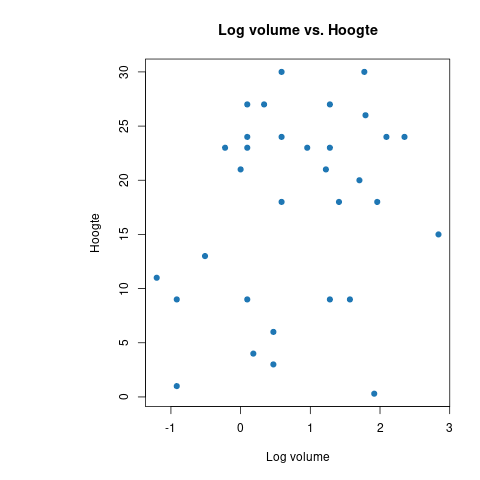
\includegraphics[width=\linewidth]{vragen/vraag3/images/scatter_plot.png}
    \captionof{figure}{Scatter plot voor log(Volume) en Hoogte.}
    \label{fig:scatter_plot}
\end{minipage}
\newline\newline\newline
\textbf{Conclusie:} Hier kunt u zien dat er een \textbf{geen} verband is tussen log(Volume) en Hoogte.
Omdat bij de scatter plot de punten niet in een rechte lijn liggen, maar willekeurig verspreid zijn, is er geen verband.
Om dit te bevestigen heb ik een correlatiecoëfficiënt berekend.
\newline\newline
Een positieve correlatiecoëfficiënt betekent een sterke positieve relatie, een negatieve correlatiecoëfficiënt betekent een sterke negatieve relatie, en een correlatiecoëfficiënt dichtbij nul geeft een zwakke of geen relatie weer.
Onderaan ziet u de resultaten van de correlatiecoëfficiënt.
\newline\newline
% insert correlation coefficient for log(Volume) and Hoogte
\begin{tabular}{l*{6}{c}r}
    Variable & Correlation Coefficient \\
    \hline
    log(Volume) en Hoogte & 0.251 \\
\end{tabular}
\newline\newline\newline
\textbf{Conclusie:} Hier kunt u zien dat de correlatiecoëfficiënt 0.251 is.
Dit betekent dat er een \textbf{zeer zwak} verband is tussen log(Volume) en Hoogte.
Ik heb ook een lineaire regressie uitgevoerd om het verband tussen log(Volume) en Hoogte aan te tonen.
Onderaan zult u de waarden terug vinden.
\newline\newline
% insert linear regression values for log(Volume) and Hoogte
\begin{tabular}{l*{6}{c}r}
    Variable & Intercept & Slope(\textit{log\_volume}) \\
    \hline
    log(Volume) en Hoogte & 15.778 & 2.193 \\
\end{tabular}
\newline\newline
De \textit{log\_volume} coëfficiënt geeft de geschatte verandering in het gemiddelde Hoogte voor een toename van één eenheid in de \textit{log\_volume} voorspellende variabele. 
In dit geval is de geschatte coëfficiënt voor \textit{log\_volume} 2.193. 
Dit betekent dat voor elke toename van één eenheid in \textit{log\_volume}, het geschatte gemiddelde Hoogte met ongeveer 2.193 eenheden stijgt.
In dit geval zou de geschatte vergelijking voor het lineaire regressiemodel zijn: $Hoogte = 15.778 + 2.193 * log\_volume$
De R-kwadraatwaarde is in dit geval 0.063. Dit wilt zeggen dat 6.3\% van de variantie in Hoogte verklaard wordt door \textit{log\_volume}.
Dat is een zeer lage waarde.
Het is niet perse dat het model onbruikbaar is, maar het kan erop wijzen dat andere factoren of variabelen een grotere invloed hebben op de variabiliteit van de afhankelijke variabele.
\newline\newline
Als laatst heb ik ook de Spearman's rank correlation coefficient berekend.
Deze is minder gevoelig voor outliers.
Onderaan ziet u de resultaten van de Spearman's rank correlation coefficient.
\newline\newline\newline
% insert spearman's rank correlation coefficient for log(Volume) and Hoogte
\begin{tabular}{l*{6}{c}r}
    Variable & Spearman's Rank Correlation Coefficient \\
    \hline
    log(Volume) en Hoogte & 0.2016 \\
\end{tabular}
\newline\newline\newline
De Spearman's rangcorrelatiecoëfficiënt van 0.2016 geeft aan dat er een zwak positief monotoon verband is tussen "\textit{log\_volume}" en "Hoogte". 
Dit betekent dat over het algemeen, wanneer de rangordes van "\textit{log\_volume}" toenemen, de rangordes van "Hoogte" ook toenemen, zij het met een zwak verband.
\newline\newline
\textbf{Conclusie:} Uit de scatter plot, correlatiecoëfficiënt, lineaire regressie en Spearman's rank correlation coefficient kunnen we besluiten dat er \textbf{zeer zwak} verband is tussen log(Volume) en Hoogte.
Het is dus niet aangeraden om uit log(Volume) de Hoogte te voorspellen.
\end{document}